\documentclass[11pt]{article}
\usepackage[utf8]{inputenc}
\usepackage[margin=0.5in, includefoot]{geometry}
\usepackage[printonlyused]{acronym}
\usepackage[bottom]{footmisc}
\usepackage{graphicx}

\graphicspath{{../figures/}}

\title{Predicting Aircraft Maneuvers with Various Flight Characteristics to Evaluate the Reliability of Non-Expert Human Observers}
\author{David R Crow, 2d Lt, USAF}
\date{16 May 2019}

\begin{document}
\frenchspacing
\maketitle

\section{Introduction}

% details of the problem domain/motivate the problem
An aircraft's maneuvers in flight are often indicated by the plane's roll, pitch, and yaw. Takeoff, for example, can be defined by a high, positive pitch and low, well-correlated values for roll and yaw. Humans, who are naturally error-prone, might misidentify an aircraft's movement when given only a visual observation of the plane. The \ac{USAF} is often concerned with the movement of its various aircraft (and those of other countries), but, in situations without access to the aircraft's flight data (to include roll, pitch, and yaw), the Air Force must rely on human observers. Presently, the \ac{USAF} does not know much about the reliability of non-expert human observers in identifying aircraft maneuvers.

% research objectives

In this research, we fit multiple \ac{ML} models to a set of aircraft characteristics generated by a flight simulator. A non-expert human observer labels each of the simulated observations with the maneuver of the aircraft at that point in time. After fitting each model, we evaluate its performance and, eventually, we identify which model best predicts the aircraft's maneuver. We then use an expert system to label the observations and compare its performance to that of our best model. In doing so, we can determine whether our human observer provides reliable testimony. We hope to generalize our results concerning reliability of observers to other domains, even if those domains are not related to the military.

% explain research gaps

Many researchers have used flight characteristics to predict other flight characteristics, aircraft type, and even the maneuver at some point in time. However, previous research, as indicated in the Related Work section, does not evaluate the reliability of its labels; instead, the researchers always assume their dataset is accurately labeled (when it is actually labeled; see \cite{Rodin1992}). In this research, we fit \ac{ML} models to our dataset much like in previous research, but we go further in comparing our model's performance to that of an expert system.

% research hypotheses
% research questions

In general, we expect our best model will be able to successfully predict aircraft maneuvers. The real significance of this research is in evaluating the accuracy of the human-labeled maneuvers. It is certainly possible that our non-expert definition of (say) turning is different from an expert's, and we wish to determine whether a model fit to \textit{our} definition is even useful in practical applications. In answering this question, we hope to illustrate why aircraft maneuvers labeled by non-experts may or may not be reliable.

% overview of machine learning task

To most effectively fit a model to our dataset, we intend to train various classifiers and conduct a performance analysis of each. The software program that generates our dataset enables fully-supervised learning; this allows us to easily determine the utility of each classifier. After fitting the best possible model to our human-labeled dataset, we compare the model to an expert system (which labels flight maneuvers based on the roll, pitch, and yaw of the aircraft) to evaluate the reliability of our labels.

% overview of dataset

We utilize the \ac{AVAS}, which the \ac{AFRL} has graciously offered to us, to generate our dataset. In layman's terms, the \ac{AVAS} is a flight simulator. At any given moment, the system computes various metrics, including airspeed, angle of attack, latitude, heading, and wind angle. For this project, we are concerned with the airplane's orientation, speed, acceleration, and altitude. The simulator is able to display these values (among others) as they change over time, and we modified the source code to enable parameter filtering and file output.

% transition paragraph

In the remainder of this report, we present our research in detail. In section two, we examine some of the related work in current literature -- and we explain why this work is insufficient for the research at hand. In section three, we describe our dataset, our model-fitting process, and our tools for analyzing and evaluating our model. In section four, we discuss our expected results and the implication of these results.

\section{Related Work}

% identify and discuss references found, indicate that the paper is well informed, show where to find more info, see what prior work I rely on, see why the research is necessary, ensure prior work is organized by themes/messages

Our primary reference material for this research is \cite{James2013}. Without it (and its accompanying resources), we likely would not have developed a sufficient understanding of relevant \ac{ML} techniques. Specifically, we reference \cite{James2013} when we have questions about dataset partitioning, the best subset and \ac{LASSO} feature selection methods, $k$-fold \ac{CV}, binary classification, \ac{KNN} classification, classification trees, and the evaluation of classifier performance.

When \cite{James2013} proves insufficient, we reference \cite{Bishop2006}. This resource describes classification in greater detail, and it also explains several classification methods not covered in \cite{James2013}. Additionally, \cite{Bishop2006} discusses multiple sampling methods that we were otherwise unaware of. Although we mostly utilize Python libraries for our sampling, this reference provides insight into why other methods might be more appropriate.

The work performed in \cite{Blanks2017} is closely-aligned with our own research. The researchers utilize an open-source dataset consisting of worldwide flight data. After collecting flight characteristics from the dataset via robust feature engineering, they predict the aircraft's type. Clearly, this research is in the same domain as our own, and we thus refer to it when evaluating our models and reporting the performance. We note here that the researchers are only concerned with objective labels (i.e., aircraft type), instead of the subjective labels we predict.

\cite{Rodin1992} is also related to our research. Like us, the researchers predict aircraft maneuvers, but they fit an artificial neural networks model to a partially-unknown dataset. However, the class labels -- although more complex than our own -- are already given by expert systems; there is little subjectivity or doubt in the labels (for those observations that actually have labels). This resource does not address the accuracy of the labels themselves.

% summary/transition paragraph

It should now be clear why this research is necessary: previous research does not evaluate questionable class labels. In other words, it does not evaluate the reliability of humans in characterizing aircraft flight maneuvers. In the following section, we detail our data and its components: the generation process, the features, and the class balance. Additionally, we explore the various features and hypothesize about the best and worst predictors of airplane maneuvers.

\section{Methodology}

% overview of the methodology

In this section, we discuss our data generation process and the resulting features and observations. Additionally, we detail the machine learning process. Specifically, we explain our model fitting procedure, to include partitioning, validation, and other \ac{ML} design choices. We also describe our evaluation procedure: how we compare different models, how we compute results, and how we analyze our results.

\subsection{Data}

% describe where the data came from

The data are generated by the \ac{AVAS}, an \ac{AFRL}-developed flying simulator that employs real-world physics and flight dynamics for \ac{USAF} research purposes. To create our dataset, we repeatedly guide the simulator through takeoff and various midair maneuvers. By documenting the relative start and end times of a turn, for example, we can easily segregate and label the relevant datapoints. By executing $n$ turns, $n$ takeoffs, and $n$ (approximately) straight and level flights, we can both balance the distribution of the three classes and generate a sizable dataset. For our own benefit, we modified the \ac{AVAS} source code so that it outputs the observations directly to a properly-formatted comma-separated values file; thus the generated file is ready for \ac{ML}.

% how many observations/features per observation in a dataframe?
% describe the nature of the features

Fortunately, the availability of the \ac{AVAS} allows us to generate arbitrary amounts of data. For this research, we claim that $5,000$ observations constitute a sufficiently-large dataset; if we wish to utilize fewer data points, we can train on and test a subset of the data. Each observation includes nine different flying metrics and a timestamp relative to the start of the simulation. The metrics include roll, pitch, and yaw (each in radians), altitude (in feet), airspeed, and vertical velocity (in feet per second), and acceleration in each of three axes (in feet per second per second). The roll and pitch values range from $-\pi$ to $\pi$ radians; yaw ranges from $0$ to $2\pi$; the altitude and airspeed are both greater than zero; the vertical velocity and accelerations are real number values. The timestamp data is only useful for labeling, so we remove it in our model fitting process.

% what info is contained in the supervised learning label?

When flying the simulator, we note the flying maneuver performed during a given time period and label all observations within this window with the maneuver in question; in doing so, we identify our truth data. Thus, our truth data are labeled according to the beliefs of the individual operating the simulator. Because this individual is not an expert in aircraft flight, we assume these labels are not always correct.

% how many classes? what is the distribution of observations?

Still, the dataset has three classes: \textit{taking off}, \textit{turning}, and \textit{cruising}. By repeating our simulations with different starting conditions, we are able to balance the presence of each of the three classes in the dataset. Because our dataset is so large, we are also able to selectively filter our data in our evaluations to achieve different class distributions (if we so desire).

% data exploration (correlations, pair plots, histograms)

In Figure \ref{fig:hist}, we show nine different histograms, one for each feature. These histograms illustrate the distribution of our features over all observations. We can see that roll, pitch, vertical velocity, y-axis acceleration, and z-axis acceleration are all relatively uniformly distributed (perhaps with some skewing). The remaining features are not uniformly distributed.

\begin{figure}[ht]
    \centering
    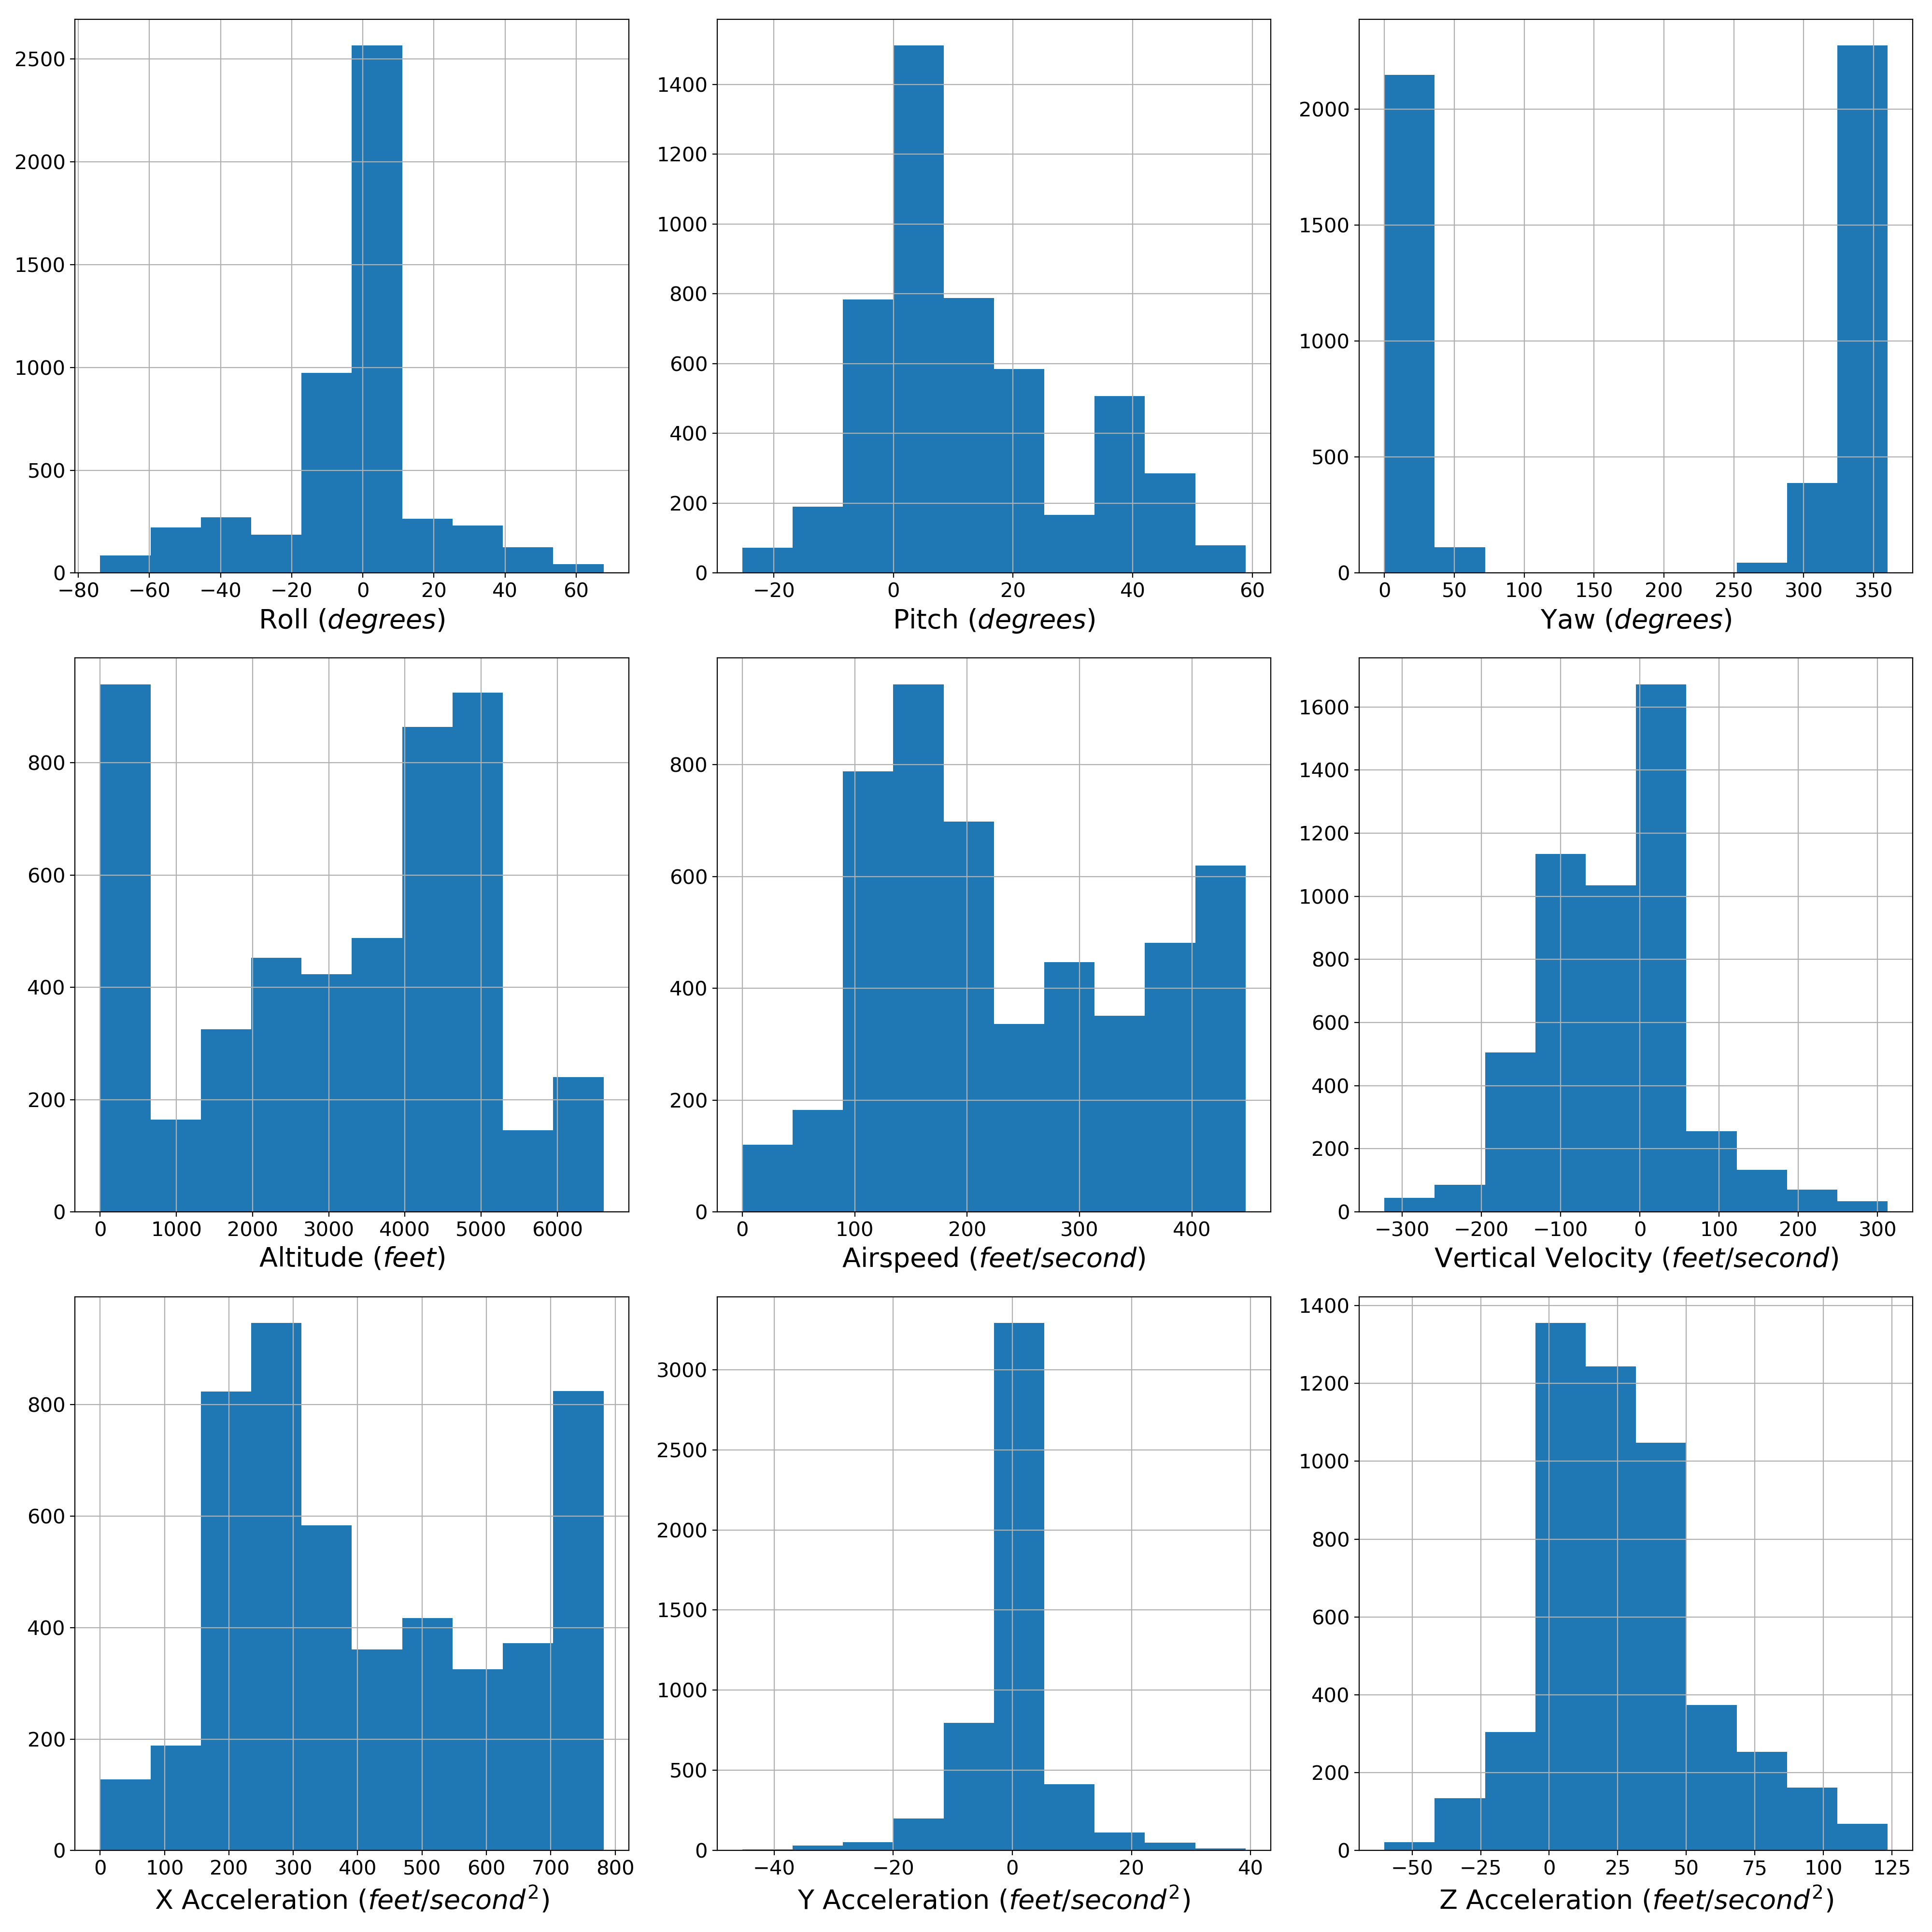
\includegraphics[scale=0.25]{all-feature-histogram.png}
    \caption{A histogram for each feature}
    \label{fig:hist}
\end{figure}

In Figure \ref{fig:3d-plots}, we plot each of three disparate groups of features on a \ac{3D} plot. Each group contains related features; for example, the first group contains roll, pitch, and yaw. As we examine the plots from left to right, we see that the boundaries between the classes grow less distinct. Thus, we predict that the features in the left plot outperform those in the middle plot, and we expect those in the middle plot to outperform those in the right plot.

\begin{figure}[ht]
    \centering
    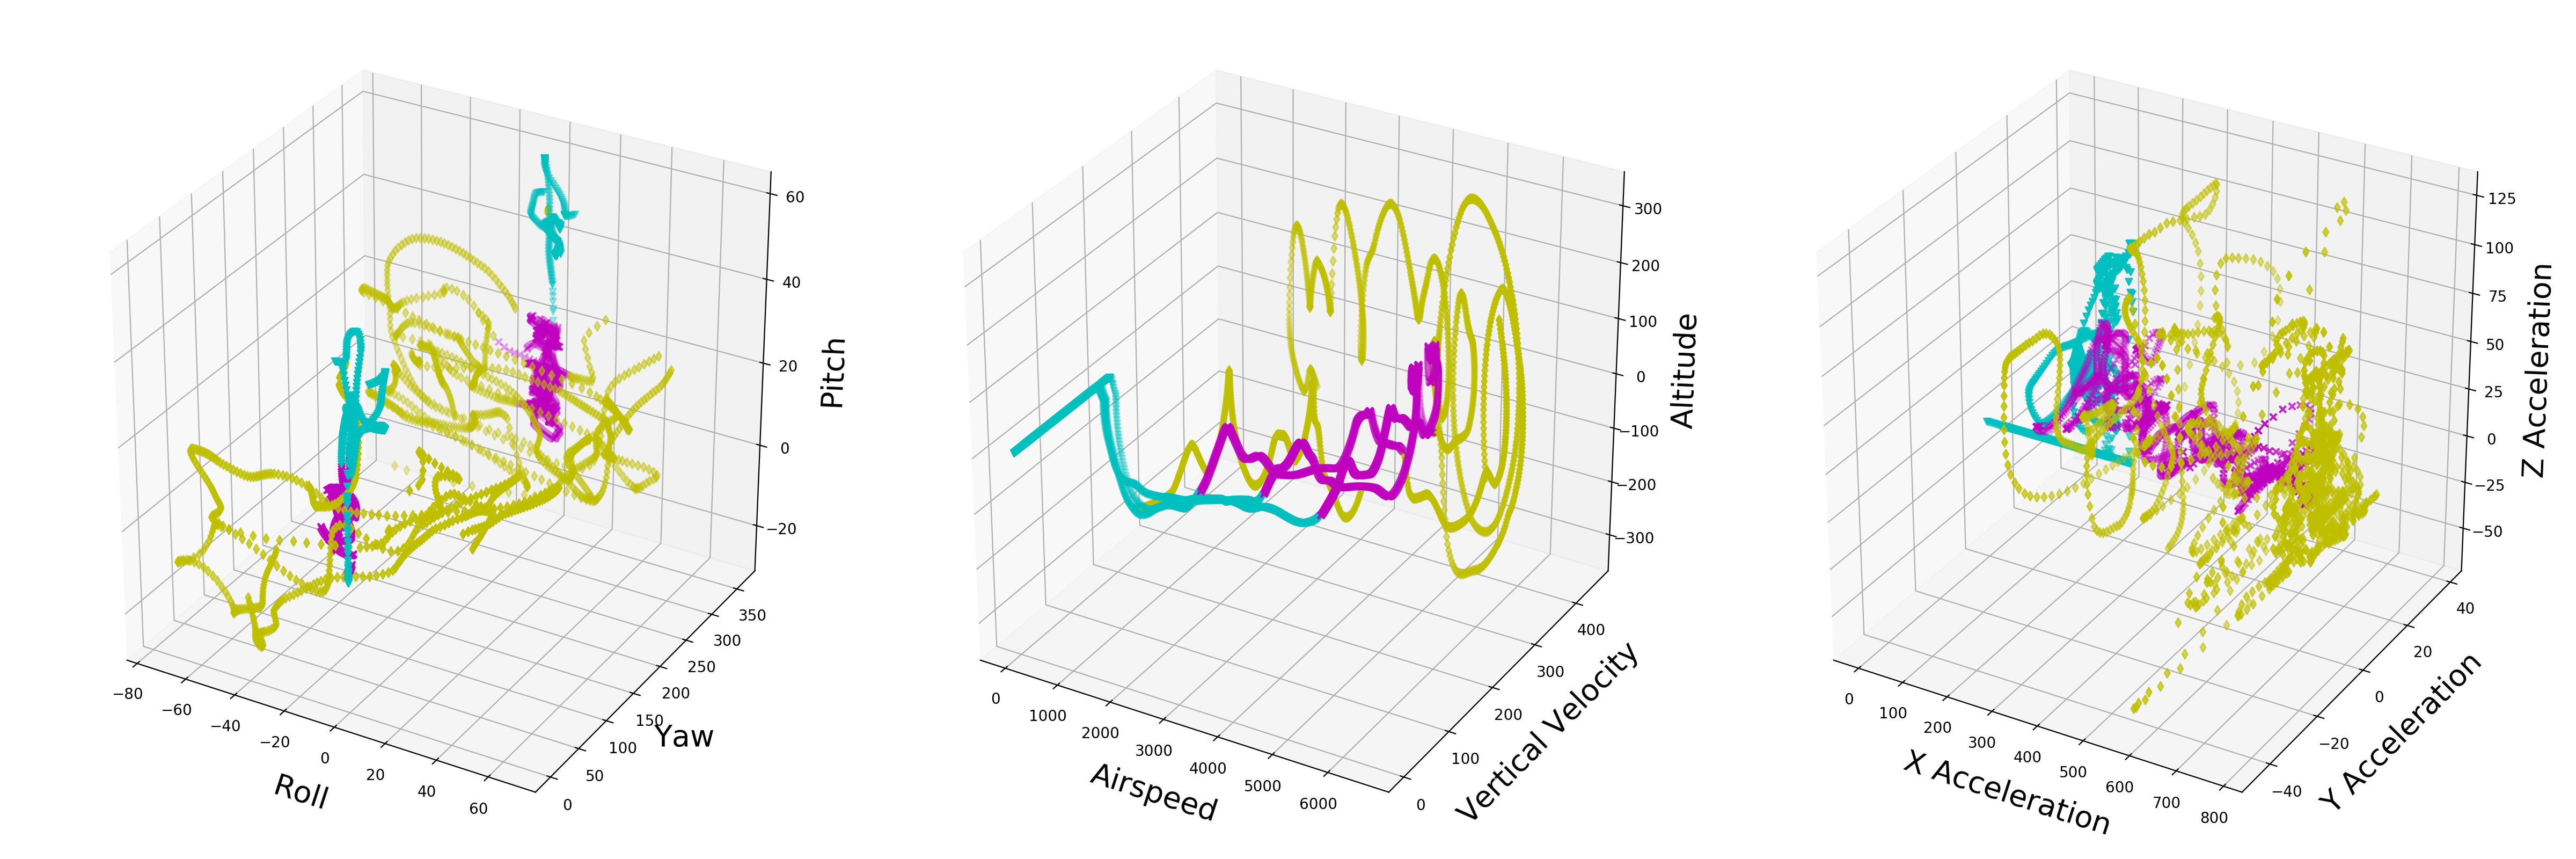
\includegraphics[scale=0.3]{3d-plots.png}
    \caption{Three-dimensional plots for groups of similar features}
    \label{fig:3d-plots}
\end{figure}

% hypothesize about important features

We expect that roll, pitch, and yaw are the best predictors of flight maneuvers specifically because the maneuvers in question are essentially \textit{defined} by roll, pitch, and yaw. We see that Figure \ref{fig:3d-plots} supports this hypothesis: clearly, the three classes are most distinct in the left plot. As a secondary objective, then, we evaluate which of the remaining features are effective predictors. As a corollary, we examine our model performance when we exclude all information about the aircraft's orientation. It is not likely a model which does not use roll, pitch, or yaw data will perform as well as one that does, but we suspect that such a model can still adequately classify flight maneuvers.

\subsection{Model Fitting}

% describe the machine learning task

Because we wish to compare the model's performance using layman-defined labels to the performance of one that uses expert-defined labels, we need to build the strongest possible classification model. For this reason, we evaluate three different classification approaches: one-versus-all binary classification \cite{James2013, Bishop2006}, \ac{KNN} classification \cite{James2013}, and the classification tree approach \cite{James2013}. In all cases, of course, our fully-labeled dataset means that we conduct fully-supervised learning.

% how are you partitioning the data into train/test sets?

To effectively evaluate the performance of both models, we partition our dataset into training and testing sets using proportional random sampling. Specifically, we sample $90\%$ of each class to build our training set; the unsampled data points constitute our test set. Because our classes are balanced in the full dataset, they are also balanced in both the training and testing sets.

% cross-validation?

When building our models, we use $k$-fold \ac{CV}. In doing so, we ensure that our models are not unnecessarily biased toward the training observations. In this research, our dataset is sufficiently large that we let $k=100$. This \ac{CV} approach certainly increases our model-building complexity (and hence the computation time), but our research requires the best model so that we can effectively evaluate the reliability of human observers; for this reason, we must minimize variance, and thus \ac{CV} is necessary. 

% regularization/feature selection?
% iteration to improve results?

\subsubsection{Binary Classification}

It is certainly possible that some of the available features are not very relevant to maneuver prediction (we note here, however, that we do not expect this to be the case). Thus, we also conduct feature selection and regularization using best subset selection and the \ac{LASSO} \cite{James2013}. We iterate over $\alpha$ values when building the \ac{LASSO} model to identify the ideal model. By utilizing both approaches, we increase our likelihood of identifying the best one-versus-all classification model. The extra computational resources required to test two methods -- instead of just one -- are negligible. In other words, we do not have much reason to \textit{not} evaluate both techniques.

\subsubsection{$k$-Nearest Neighbors}

Because our feature ranges are varied, and because \ac{KNN} is sensitive to this, we scale each of our features before building a model; in doing so, we reduce unnecessary sensitivity. Additionally, we iterate over values for $k$ until we find the the optimal value. In performing $k$-fold \ac{CV}, we ensure our choice of $k$ in \ac{KNN} is correct.

\subsubsection{Classification Trees}

In our classification tree approach, we apply a version of feature selection: random forests. Specifically, we employ a random forest approach to reduce variance in our results. Each tree in a random forest operates on a subset of the available features, so we claim that this method is akin to the binary classification feature selection methods. Like in the binary classification approach, we iterate over possible values for $m$, where $m$ is the size of the available predictor subset; this allows for the best possible model.

\subsection{Model Evaluation \& Analysis}

% comparing models? improving on existing models?

By tuning our models and their parameters, we identify the single best classifier for our dataset. We then compare this optimal model to a simple, expert predictor based on roll, pitch, and yaw. Large discrepancies in performance of the two systems indicate that the observations are mislabeled. In other words, said discrepancies imply that non-experts are not reliable in characterizing aircraft maneuvers. Small discrepancies, on the other hand, illustrate that our labels are accurate in most cases.

% evaluation of model or hyperparameter choices?
% confusion matrices? ROC/AUC? accuracy? precision? class imbalances?
% multiple repetition?
% plan for evaluating errors/residuals?

To actually determine our best model and compare it against the expert system, we need a reliable evaluation procedure. In this research, we generate a confusion matrix for each class; we then plot a \ac{ROC} curve for each matrix. By computing the \ac{AUC} for each \ac{ROC} curve and averaging the \ac{AUC} values for each model, we can easily compare model performance. Of course, we must evaluate each of our models (that is, each of our model and parameter value combinations) in this way, but repeating these computations is trivial.

To validate our performance analyses, we also consider other metrics that use the confusion matrices (e.g., accuracy, recall, F1-score). Because these metrics are application-dependent, we must conduct further analysis of the data before deciding which metric is best.

% transition paragraph

We have now described how we evaluate the classification performance of our models. In the following section, we detail the results of our model evaluation. Specifically, we describe what each of various potential results might indicate about our system and about other, less-related systems, and we then discuss which of these outcomes is most likely.

\section{Expected Results}

% overview

\renewcommand*{\thefootnote}{\fnsymbol{footnote}}
If the expert system performs significantly\footnotemark[2] better than our best possible model, then we know that our layman-applied labels are unreliable. We imagine this conclusion can apply to more than just aircraft maneuvers (for example, in evaluating the validity of crime-scene witness testimony). If, on the other hand, we find that our best model performs much like the expert system, then we can conclude that a human observer does not need expert knowledge to accurately classify aircraft maneuvers. Again, this can likely be generalized so as to apply to other situations. In this research, we expect two outcomes:

\begin{enumerate}
    \item Our best model accurately predicts the class of observations within our test set, and
    \item Our best model fails to achieve the same performance as the expert system.
\end{enumerate}

\noindent Because each of our $10$ features seem capable of predicting an aircraft's activity (some moreso than others, of course), we believe that even small subsets of the features can prove useful in our classification problem. However, we also believe that our human class-labeler cannot adequately identify the classes, especially when the boundaries are not clear. For example, our observer may classify a maneuver as \textit{cruising}, when, according to the expert system, the aircraft is actually \textit{turning}. We expect our observer to correctly classify most observations, but we also expect that the number of misclassifications is nontrivial. Further investigation of our dataset is required, as is the actual model-fitting process.

\footnotetext[2]{After we spend more time with the data, we expect to define what exactly constitutes a significant improvement.}

\pagebreak
\section*{List of Acronyms}
\begin{acronym}[LASSO]
    \acro{AFRL}{Air Force Research Lab}
    \acro{AUC}{area under the curve}
    \acro{AVAS}{Avionics Vulnerability Assessment System}
    \acro{CV}{cross-validation}
    \acro{EDM}{empirical domain modeling}
    \acro{IDS}{Intrusion Detection System}
    \acro{KNN}{$k$-nearest neighbors}
    \acro{LASSO}{least absolute shrinkage and selection operator}
    \acro{ML}{machine learning}
    \acro{ROC}{receiver operating characteristics}
    \acro{USAF}{United States Air Force}
    \acro{3D}{three-dimensional}
\end{acronym}

\bibliographystyle{ieeetr}
\bibliography{references}

\end{document}